\chapter{Program Logic and Indefinite Loops}

\section{Phần dịch trang 0 đến 10}
Chương 5 Logic chương trình và Vòng lặp vô định (Indefinite Loops)

\subsection*{5.1 Vòng lặp while}
\begin{itemize}
    \item Vòng lặp tìm ước số nhỏ nhất
    \item Số ngẫu nhiên (Random Numbers)
    \item Mô phỏng (Simulations)
    \item Vòng lặp do/while
\end{itemize}

\subsection*{5.2 Thuật toán Fencepost}
\begin{itemize}
    \item Fencepost với if
    \item Vòng lặp Sentinel (Sentinel Loops)
\end{itemize}

\subsection*{5.3 Kiểu dữ liệu boolean}
\begin{itemize}
    \item Các toán tử logic (Logical Operators)
    \item Đánh giá ngắn mạch (Short-Circuited Evaluation)
    \item Biến boolean và Cờ hiệu (Flags)
    \item Thiền Boolean (Boolean Zen)
    \item Phủ định biểu thức Boolean
\end{itemize}

\subsection*{5.4 Lỗi người dùng}
\begin{itemize}
    \item Kỹ thuật Scanner Lookahead
    \item Xử lý lỗi người dùng
\end{itemize}

\subsection*{5.5 Khẳng định (Assertions) và Logic chương trình}
\begin{itemize}
    \item Lập luận về các Khẳng định
    \item Ví dụ chi tiết về Khẳng định
\end{itemize}

\subsection*{5.6 Nghiên cứu điển hình: NumberGuess}
\begin{itemize}
    \item Phiên bản đầu tiên không có gợi ý
    \item Phiên bản ngẫu nhiên có gợi ý
    \item Phiên bản hoàn chỉnh chống lỗi (Robust Version)
\end{itemize}

\subsection*{Giới thiệu}
Chương này bắt đầu bằng việc nghiên cứu một cấu trúc mới gọi là vòng lặp \texttt{while}, cho phép bạn lặp lại một số lần vô định (indefinite number of times). Vòng lặp \texttt{while} sẽ cho phép bạn giải quyết một lớp bài toán lập trình mới mà trong đó bạn không biết trước mình muốn vòng lặp thực thi bao nhiêu lần. Ví dụ, các chương trình chơi game thường liên quan đến vòng lặp \texttt{while} vì không thể biết trước người dùng sẽ chơi game như thế nào. Bởi vì chúng ta sẽ khám phá các chương trình trò chơi, chúng ta cũng sẽ tìm hiểu cách tạo số ngẫu nhiên bên trong một chương trình Java. Chúng ta cũng sẽ khám phá một lớp thuật toán khác được gọi là thuật toán fencepost (thuật toán hàng rào) thường xuất hiện trong các tác vụ lập trình vòng lặp.

Sau đó, chương này sẽ thảo luận về kiểu dữ liệu nguyên thủy thứ tư mà chúng ta sẽ nghiên cứu chi tiết, \texttt{boolean}. Kiểu \texttt{boolean} được sử dụng để lưu trữ thông tin logic (đúng/sai - true/false). Khi bạn đã hiểu chi tiết về kiểu \texttt{boolean}, bạn sẽ có thể viết các vòng lặp phức tạp liên quan đến nhiều điều kiện kiểm tra.

Tiếp theo, chúng ta sẽ xem xét ngắn gọn chủ đề quan trọng về xử lý lỗi của người dùng.

Chương này kết thúc bằng cuộc thảo luận về các khẳng định (assertions). Bằng cách sử dụng các khẳng định, bạn có thể lập luận về các thuộc tính hình thức của chương trình (điều gì là đúng tại các thời điểm khác nhau trong quá trình thực thi chương trình).

\subsection*{5.1 Vòng lặp while}
Các vòng lặp \texttt{for} mà chúng ta đã viết từ Chương 2 là các vòng lặp khá đơn giản, thực thi một số lần có thể dự đoán được. Hãy nhớ rằng chúng ta gọi chúng là vòng lặp xác định (definite loops) vì chúng ta biết chính xác chúng sẽ thực thi bao nhiêu lần trước khi vòng lặp bắt đầu chạy. Bây giờ chúng ta muốn chuyển sự chú ý sang các vòng lặp vô định (indefinite loops), thực thi một số lần chưa biết trước. Vòng lặp vô định thường xuất hiện trong các chương trình tương tác và xử lý tệp. Ví dụ, bạn không biết trước một người dùng muốn chơi một trò chơi bao nhiêu lần, và bạn sẽ không biết trước khi xem một tệp chính xác lượng dữ liệu mà nó lưu trữ.

Vòng lặp \texttt{while} là vòng lặp vô định đầu tiên chúng ta sẽ nghiên cứu. Nó có cú pháp như sau:

\begin{verbatim}
while (<test>) {
    <statement>;
    <statement>;
     ...
    <statement>;
}
\end{verbatim}

Sơ đồ trong Hình 5.1 chỉ ra luồng điều khiển của vòng lặp \texttt{while}. Vòng lặp thực hiện kiểm tra điều kiện của nó và nếu điều kiện đánh giá là \texttt{true}, nó sẽ thực thi các câu lệnh được kiểm soát. Nó liên tục kiểm tra và thực thi nếu điều kiện đánh giá là \texttt{true}. Chỉ khi điều kiện đánh giá là \texttt{false} thì vòng lặp mới kết thúc.

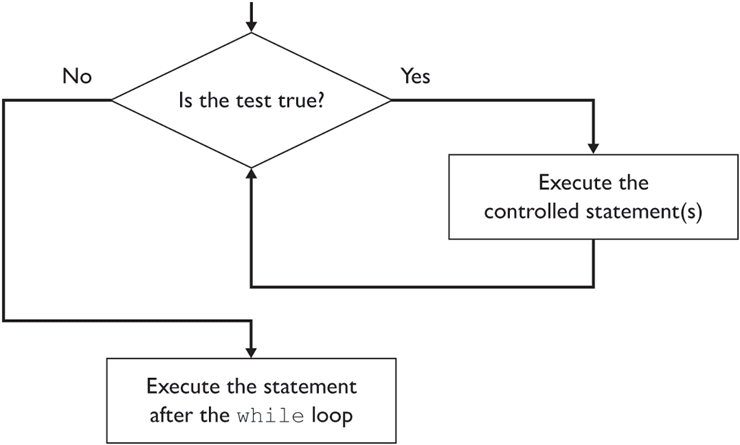
\includegraphics[max width=\linewidth]{Pictures/ch05_p4_img0.png}
\\
\textit{Hình 5.1: Luồng hoạt động của vòng lặp while}

Như Hình 5.1 chỉ ra, vòng lặp \texttt{while} thực hiện kiểm tra điều kiện ở phần đầu của vòng lặp, trước khi thân vòng lặp được thực thi. Một vòng lặp \texttt{while} sẽ không thực thi các câu lệnh được kiểm soát của nó nếu điều kiện của nó đánh giá là \texttt{false} ngay trong lần đầu tiên nó được đánh giá.

Dưới đây là một ví dụ về vòng lặp \texttt{while}:

\begin{verbatim}
int number = 1;
while (number <= 200) {
    number = number * 2;
}
\end{verbatim}

Vòng lặp này khởi tạo một biến số nguyên tên là \texttt{number} bằng 1 và sau đó nhân đôi nó trong khi nó nhỏ hơn hoặc bằng 200. Nhìn bề ngoài, hoạt động này tương tự như việc sử dụng câu lệnh \texttt{if}:

\begin{verbatim}
int number = 1;
if (number <= 200) {
    number = number * 2;
}
\end{verbatim}

Sự khác biệt giữa hai dạng này là vòng lặp \texttt{while} thực thi nhiều lần, lặp lại cho đến khi điều kiện kiểm tra đánh giá là \texttt{false}. Câu lệnh \texttt{if} chỉ thực thi câu lệnh nhân đôi một lần duy nhất, để lại \texttt{number} bằng 2. Vòng lặp \texttt{while} thực thi câu lệnh nhân đôi lặp đi lặp lại, với \texttt{number} nhận các giá trị 1, 2, 4, 8, 16, 32, 64, 128, và 256. Vòng lặp không dừng thực thi cho đến khi điều kiện kiểm tra đánh giá là \texttt{false}. Nó thực thi câu lệnh gán tám lần và kết thúc khi \texttt{number} được đặt thành giá trị 256 (lũy thừa đầu tiên của 2 lớn hơn 200).

Dưới đây là một vòng lặp \texttt{while} chứa hai câu lệnh:

\begin{verbatim}
int number = 1;
while (number <= max) {
    System.out.println("Hi there");
    number++;
}
\end{verbatim}

Vòng lặp \texttt{while} này gần như giống hệt với vòng lặp \texttt{for} sau:

\begin{verbatim}
for (int number = 1; number <= max; number++) {
    System.out.println("Hi there");
}
\end{verbatim}

Sự khác biệt duy nhất giữa hai vòng lặp này là phạm vi hoạt động (scope) của biến \texttt{number}. Trong vòng lặp \texttt{while}, \texttt{number} được khai báo trong phạm vi bên ngoài vòng lặp. Trong vòng lặp \texttt{for}, \texttt{number} được khai báo bên trong vòng lặp.

\subsection*{Vòng lặp tìm ước số nhỏ nhất}
Giả sử bạn muốn tìm ước số nhỏ nhất của một số khác 1. Bảng 5.1 đưa ra các ví dụ về những gì bạn đang tìm kiếm.

\textit{Bảng 5.1: Ví dụ về các ước số}

Dưới đây là mô tả bằng mã giả (pseudocode) về cách bạn có thể tìm giá trị này:

\begin{verbatim}
bắt đầu divisor tại 2.
while (giá trị hiện tại của divisor không chia hết) {
    tăng divisor.
}
\end{verbatim}

Bạn không bắt đầu \texttt{divisor} tại 1 vì bạn đang tìm kiếm ước số đầu tiên lớn hơn 1. Để tinh chỉnh mã giả này, bạn phải rõ ràng hơn về điều gì làm cho một ước số "chia hết". Một ước số của một số sẽ không có số dư khi số đó được chia cho ước số đó. Bạn có thể viết lại quy tắc này dưới dạng mã giả sau:

\begin{verbatim}
bắt đầu divisor tại 2.
while (số dư của number/divisor không bằng 0) {
    tăng divisor.
}
\end{verbatim}

Bài toán này có thể được giải quyết bằng cách sử dụng toán tử chia lấy dư \texttt{\%}, toán tử này cho biết số dư của phép chia số nguyên. Vòng lặp \texttt{while} sau đây thực hiện tác vụ đó:

\begin{verbatim}
int divisor = 2;
while (number % divisor != 0) {
    divisor++;
}
\end{verbatim}

Một vấn đề mà bạn chắc chắn sẽ gặp phải khi viết vòng lặp \texttt{while} là vòng lặp vô hạn (infinite loop) khét tiếng. Hãy xem xét đoạn mã sau:

\begin{verbatim}
int number = 1;
while (number > 0) {
    number++;
}
\end{verbatim}

Bởi vì \texttt{number} bắt đầu là một giá trị dương và vòng lặp làm cho nó lớn hơn, vòng lặp này sẽ tiếp tục vô tận. Bạn phải cẩn thận khi xây dựng các vòng lặp \texttt{while} của mình để tránh các tình huống mà một đoạn mã sẽ không bao giờ kết thúc quá trình thực thi. Mỗi khi bạn viết một vòng lặp \texttt{while}, bạn nên cân nhắc xem khi nào và làm thế nào nó sẽ kết thúc thực thi.

\subsection*{LỖI LẬP TRÌNH PHỔ BIẾN: Vòng lặp vô hạn}
Viết một vòng lặp \texttt{while} không bao giờ kết thúc là điều tương đối dễ mắc phải. Một lý do khiến lỗi này dễ xảy ra là vòng lặp \texttt{while} không có bước cập nhật trong phần đầu của nó như vòng lặp \texttt{for}. Điều quan trọng là lập trình viên phải đưa vào một bước cập nhật chính xác vì bước này là cần thiết để cuối cùng làm cho điều kiện kiểm tra của vòng lặp bị thất bại (trả về \texttt{false}).

Hãy xem xét đoạn mã sau, được thiết kế để yêu cầu người dùng nhập một số và liên tục in ra số đó được giảm đi một nửa cho đến khi đạt đến 0. Lần thử đầu tiên này không biên dịch được:

\begin{verbatim}
Scanner console = new Scanner(System.in);
System.out.print("Type a number: "); 
 
// đoạn mã này không biên dịch được
while (number > 0) {
    int number = console.nextInt();
}
\end{verbatim}
\section{Phần dịch trang 10 đến 20}
\begin{verbatim}
    System.out.println(number / 2);
}
\end{verbatim}

Vấn đề với đoạn mã trước đó là biến \texttt{number} cần phải nằm trong phạm vi hiệu lực (scope) trong quá trình kiểm tra điều kiện của vòng lặp (loop), vì vậy nó không thể được khai báo bên trong vòng lặp. Một nỗ lực không chính xác để khắc phục lỗi biên dịch này là cắt và dán dòng khởi tạo \texttt{number} ra bên ngoài vòng lặp:

\begin{verbatim}
// đoạn mã này có một vòng lặp vô hạn
int number = console.nextInt(); // được di chuyển ra ngoài vòng lặp 
 
while (number > 0) {
    System.out.println(number / 2);
}
\end{verbatim}

Phiên bản này của đoạn mã có một vòng lặp vô hạn (infinite loop); nếu vòng lặp được bắt đầu, nó sẽ không bao giờ kết thúc. Vấn đề này phát sinh vì không có câu lệnh cập nhật nào bên trong thân vòng lặp \texttt{while} để thay đổi giá trị của \texttt{number}. Nếu \texttt{number} lớn hơn 0, vòng lặp sẽ liên tục in ra giá trị của nó và kiểm tra điều kiện vòng lặp, và điều kiện đó sẽ luôn trả về kết quả là \texttt{true}.

Phiên bản dưới đây của đoạn mã sẽ giải quyết vấn đề vòng lặp vô hạn. Vòng lặp chứa một bước cập nhật trong mỗi lần lặp để chia đôi số nguyên và lưu trữ giá trị mới của nó. Nếu số nguyên chưa đạt đến giá trị 0, vòng lặp sẽ tiếp tục:

\begin{verbatim}
// đoạn mã này hoạt động chính xác
int number = console.nextInt(); // được di chuyển ra ngoài vòng lặp
while (number > 0) {
    number = number / 2; // bước cập nhật: chia đôi
    System.out.println(number);
}
\end{verbatim}

Ý tưởng cốt lõi là thân của mỗi vòng lặp \texttt{while} đều nên chứa đoạn mã để cập nhật các số hạng được kiểm tra trong điều kiện vòng lặp. Nếu điều kiện vòng lặp \texttt{while} kiểm tra giá trị của một biến, thân vòng lặp nên gán lại một giá trị mới có ý nghĩa cho biến đó.

\subsection*{Số ngẫu nhiên (Random Numbers)}

Chúng ta thường muốn các chương trình của mình thể hiện các hành vi có vẻ ngẫu nhiên. Ví dụ, chúng ta muốn các chương trình trò chơi tạo ra một con số để người dùng đoán, xáo trộn một bộ bài, chọn một từ trong danh sách để người dùng đoán, v.v. Bản chất của các chương trình máy tính là có thể dự đoán được và không ngẫu nhiên. Nhưng chúng ta có thể tạo ra các giá trị có vẻ như ngẫu nhiên. Những giá trị như vậy được gọi là giả ngẫu nhiên (pseudorandom) vì chúng được tạo ra bằng thuật toán.

\textbf{Số giả ngẫu nhiên (Pseudorandom Numbers)}
\begin{quote}
Những con số mà mặc dù được bắt nguồn từ các thuật toán có thể dự đoán trước và được xác định rõ ràng, nhưng lại mô phỏng các đặc tính của các con số được chọn một cách ngẫu nhiên.
\end{quote}

Java cung cấp một vài cơ chế để có được các số giả ngẫu nhiên. Một lựa chọn là gọi phương thức \texttt{random} từ lớp \texttt{Math} để lấy một giá trị ngẫu nhiên kiểu \texttt{double} có thuộc tính sau:
\[
0.0 \le \text{Math.random()} < 1.0
\]
Phương thức này cung cấp một cách nhanh chóng và dễ dàng để có được một số ngẫu nhiên, và bạn có thể sử dụng phép nhân để thay đổi phạm vi của các số mà phương thức tạo ra. Java cũng cung cấp một lớp gọi là \texttt{Random} giúp sử dụng dễ dàng hơn. Nó được bao gồm trong gói \texttt{java.util}, vì vậy bạn phải khai báo \texttt{import} ở đầu chương trình để sử dụng nó.

Các đối tượng \texttt{Random} có một vài phương thức hữu ích liên quan đến việc tạo số giả ngẫu nhiên, được liệt kê trong Bảng 5.2. Mỗi khi bạn gọi một trong những phương thức này, Java sẽ tạo và trả về một số ngẫu nhiên mới thuộc kiểu dữ liệu được yêu cầu.

\textbf{Bảng 5.2 Các phương thức hữu ích của đối tượng Random}

Để tạo các số ngẫu nhiên, trước tiên bạn cần xây dựng một đối tượng \texttt{Random}:
\begin{verbatim}
Random r = new Random();
\end{verbatim}
Sau đó, bạn có thể gọi phương thức \texttt{nextInt} của nó, truyền vào một số nguyên tối đa. Con số trả về sẽ nằm trong khoảng từ 0 (bao gồm) đến giá trị tối đa đó (không bao gồm). Ví dụ: nếu bạn gọi \texttt{nextInt(100)}, bạn sẽ nhận được một số từ 0 đến 99. Bạn có thể cộng thêm 1 vào số đó để có được phạm vi từ 1 đến 100.

Tương tác JShell sau đây tạo ra một đối tượng \texttt{Random} và sử dụng nó để tạo ra một vài số ngẫu nhiên từ 1 đến 10. Lưu ý rằng mỗi lần gọi \texttt{nextInt} đều tạo ra một số nguyên ngẫu nhiên mới:
\begin{verbatim}
jshell> Random r = new Random();
r ==> java.util.Random@5c7fa833 
 
jshell> r.nextInt(10)
$2 ==> 2 
 
jshell> r.nextInt(10)
$3 ==> 9 
 
jshell> r.nextInt(10)
$4 ==> 9 
 
jshell> r.nextInt(10)
$5 ==> 0 
 
jshell> r.nextInt(10)
$6 ==> 5
\end{verbatim}

Hãy cùng xem một chương trình đơn giản chọn các số từ 1 đến 10 cho đến khi một số cụ thể xuất hiện. Chúng ta sẽ sử dụng một đối tượng \texttt{Random} để tạo ra các số giả ngẫu nhiên.

Vòng lặp của chúng ta sẽ trông giống như thế này (trong đó \texttt{number} là giá trị mà người dùng yêu cầu chúng ta tạo ra):
\begin{verbatim}
int result;
while (result != number) {
    result = r.nextInt(10) + 1; // số ngẫu nhiên từ 1-10

    System.out.println("next number = " + result);
}
\end{verbatim}

Lưu ý rằng chúng ta phải khai báo biến \texttt{result} bên ngoài vòng lặp \texttt{while}, bởi vì \texttt{result} xuất hiện trong phần kiểm tra điều kiện của vòng lặp \texttt{while}. Đoạn mã trên có hướng tiếp cận đúng, nhưng Java sẽ không chấp nhận nó. Đoạn mã sẽ tạo ra một thông báo lỗi rằng biến \texttt{result} có thể chưa được khởi tạo. Đây là một ví dụ về một vòng lặp cần được mồi (priming).

\textbf{Mồi vòng lặp (Priming a Loop)}
\begin{quote}
Khởi tạo các biến trước một vòng lặp để "mồi bơm" và đảm bảo rằng vòng lặp sẽ được thực thi.
\end{quote}

Chúng ta muốn đặt biến \texttt{result} thành một giá trị nào đó để khiến vòng lặp được thực thi, nhưng giá trị cụ thể không quan trọng miễn là nó đưa chúng ta vào được trong vòng lặp. Tuy nhiên, chúng ta cần cẩn thận không đặt nó thành giá trị mà người dùng muốn chúng ta tạo ra. Trong chương trình này, chúng ta đang làm việc với các giá trị từ 1 đến 10, vì vậy chúng ta có thể đặt \texttt{result} thành một giá trị như -1 vốn rõ ràng nằm ngoài phạm vi số này. Đôi khi chúng ta gọi đây là một giá trị "giả" (dummy value) vì chúng ta không thực sự xử lý nó. Ở phần sau của chương trình này, chúng ta sẽ thấy một biến thể của vòng lặp \texttt{while} không yêu cầu kiểu mồi này.

Dưới đây là giải pháp chương trình hoàn chỉnh:
\begin{verbatim}
 1 // Chọn các số ngẫu nhiên từ 1-10 cho đến khi chọn được giá trị đã cho.
 2 import java.util.*;
 3 
 4 public class Pick {
 5     public static void main(String[] args) {
 6         System.out.println("This program picks numbers from");
 7         System.out.println("1 to 10 until a particular");
 8         System.out.println("number comes up.");
 9         System.out.println();
10
11         Scanner console = new Scanner(System.in);
12         Random r = new Random();
13
14         System.out.print("Pick a number between 1 and 10--> ");
15         int number = console.nextInt();
16
17         int result = -1; // đặt thành -1 để đảm bảo chúng ta vào vòng lặp
18         int count = 0;
19         while (result != number) {
20             result = r.nextInt(10) + 1; // số ngẫu nhiên từ 1-10

21             System.out.println("next number = " + result);
22             count++;
23         }
24         System.out.println("Your number came up after " +
25                            count + " times");
26     }
27 }
\end{verbatim}

Tùy thuộc vào chuỗi số được trả về bởi đối tượng \texttt{Random}, chương trình có thể kết thúc việc chọn số đã cho một cách nhanh chóng, như trong kết quả chạy mẫu sau:
\begin{verbatim}
This program picks numbers from 
1 to 10 until a particular 
number comes up. 
 
Pick a number between 1 and 10--> 2 
next number = 7 
next number = 8 
next number = 2 
Your number came up after 3 times
\end{verbatim}

Cũng có khả năng chương trình sẽ mất một khoảng thời gian để chọn được số đó, như trong kết quả chạy mẫu dưới đây:
\begin{verbatim}
This program picks numbers from 
1 to 10 until a particular 
number comes up. 
 
Pick a number between 1 and 10--> 10 
next number = 9 
next number = 7 
next number = 7 
next number = 5 
next number = 8 
next number = 8 
next number = 1 
next number = 5 
next number = 1 
next number = 9 
next number = 7 
next number = 10 
Your number came up after 12 times
\end{verbatim}

\subsection*{LỖI LẬP TRÌNH PHỔ BIẾN}
\textit{Sử dụng sai đối tượng Random}

Một đối tượng \texttt{Random} sẽ chọn một số nguyên ngẫu nhiên mới mỗi khi phương thức \texttt{nextInt} được gọi. Khi sinh viên cố gắng tạo ra một giá trị ngẫu nhiên có điều kiện ràng buộc, chẳng hạn như một số lẻ, đôi khi họ viết nhầm đoạn mã như sau:
\begin{verbatim}
// đoạn mã này chứa một lỗi (bug)
Random r = new Random(); 
 
if (r.nextInt() % 2 == 0) {
    System.out.println("Even number: " + r.nextInt());
} else {
    System.out.println("Odd number: " + r.nextInt());
}
\end{verbatim}

Đoạn mã trên thất bại trong nhiều trường hợp vì đối tượng \texttt{Random} tạo ra một số nguyên ngẫu nhiên để sử dụng trong kiểm tra điều kiện \texttt{if/else}, và sau đó lại tạo một số khác để sử dụng trong bất kỳ câu lệnh \texttt{println} nào được chọn để thực thi. Ví dụ, kiểm tra điều kiện \texttt{if} có thể nhận được giá trị ngẫu nhiên là 47 từ đối tượng \texttt{Random}. Phép thử sẽ thấy rằng $47 \% 2$ không bằng 0, vì vậy đoạn mã sẽ chuyển sang câu lệnh \texttt{else}. Câu lệnh \texttt{println} sau đó sẽ thực thi một lệnh gọi khác tới \texttt{nextInt}, lệnh này sẽ trả về một con số hoàn toàn khác (chẳng hạn như 128). Kết quả đầu ra của đoạn mã khi đó sẽ là câu lệnh kỳ lạ sau:
\section{Phần dịch trang 20 đến 30}
Số lẻ: 128

Giải pháp cho vấn đề này là lưu trữ số nguyên được chọn ngẫu nhiên vào một biến và chỉ gọi lại \texttt{nextInt} khi thực sự cần một số ngẫu nhiên khác. Đoạn mã sau đây thực hiện tác vụ này:

\begin{verbatim}
// đoạn mã này hoạt động chính xác
Random r = new Random();
int n = r.nextInt(); // lưu số ngẫu nhiên vào một biến
if (n % 2 == 0) {
    System.out.println("Even number: " + n);
} else {
    System.out.println("Odd number: " + n);
}
\end{verbatim}

\subsection*{Mô phỏng (Simulations)}

Khoa học và kỹ thuật truyền thống đòi hỏi nhiều sự tương tác trong thế giới thực. Các nhà khoa học tiến hành thực nghiệm để kiểm tra các giả thuyết của họ và các kỹ sư xây dựng các mẫu thử (prototypes) để thử nghiệm các thiết kế của mình. Nhưng ngày càng có nhiều nhà khoa học và kỹ sư tìm đến máy tính như một cách để tăng năng suất bằng cách chạy các mô phỏng (simulations) trước nhằm khám phá các khả năng, trước khi họ tiến hành một thực nghiệm thực tế hoặc xây dựng một mẫu thử thực tế. Một nhà khoa học máy tính nổi tiếng tên là Jeanette Wing đã lập luận rằng việc tăng cường sử dụng tính toán này của các nhà khoa học và kỹ sư sẽ dẫn đến tư duy máy tính (computational thinking) được xem là nền tảng, giống như cách mà việc đọc, viết và làm toán được coi là nền tảng ngày nay.

Dưới góc độ lập trình, hai thành phần chính trong một mô phỏng là các số giả ngẫu nhiên (pseudorandom numbers) và các vòng lặp (loops). Một số mô phỏng có thể được viết bằng cách sử dụng vòng lặp \texttt{for}, nhưng thông thường chúng ta sử dụng vòng lặp \texttt{while} vì mô phỏng cần được chạy vô hạn cho đến khi một điều kiện nào đó được thỏa mãn.

Là một ví dụ đơn giản, chúng ta hãy xem cách mô phỏng việc tung hai con xúc xắc cho đến khi tổng số điểm của chúng bằng 7. Chúng ta có thể sử dụng một đối tượng \texttt{Random} để mô phỏng các con xúc xắc, gọi nó một lần cho mỗi con xúc xắc. Chúng ta muốn lặp lại cho đến khi tổng bằng 7 và có thể in ra các lần tung khác nhau xuất hiện khi chạy mô phỏng. Dưới đây là một thử nghiệm đầu tiên khá tốt:

\begin{verbatim}
Random r = new Random();
while (sum != 7) {
    // tung xúc xắc một lần
    int roll1 = r.nextInt(6) + 1;
    int roll2 = r.nextInt(6) + 1;
    int sum = roll1 + roll2;
    System.out.println(roll1 + " + " + roll2 + " = " + sum);
}
\end{verbatim}

Đoạn mã trên tạo ra lỗi trình biên dịch sau:

\begin{verbatim}
Dice.java:7: error: cannot find symbol
symbol : variable sum
location: class Dice
    while (sum != 7) {
              ^
1 error
\end{verbatim}

Vấn đề là điều kiện kiểm tra vòng lặp \texttt{while} tham chiếu đến biến \texttt{sum}, nhưng biến đó lại được khai báo bên trong thân vòng lặp. Chúng ta không thể khai báo biến trong phạm vi bên trong (inner scope) vì chúng ta cần tham chiếu đến nó trong điều kiện kiểm tra vòng lặp. Vì vậy, chúng ta phải chuyển khai báo biến lên trước vòng lặp. Chúng ta cũng phải gán cho biến một giá trị ban đầu để đảm bảo rằng nó sẽ đi vào vòng lặp. Đoạn mã này là một ví dụ khác về thời điểm chúng ta cần chuẩn bị trước cho vòng lặp (prime the loop):

\begin{verbatim}
Random r = new Random();
int sum = 0; // đặt thành 0 để đảm bảo chúng ta vào vòng lặp
while (sum != 7) {
    // tung xúc xắc một lần
    int roll1 = r.nextInt(6) + 1;
    int roll2 = r.nextInt(6) + 1;
    sum = roll1 + roll2;
    System.out.println(roll1 + " + " + roll2 + " = " + sum);
}
\end{verbatim}

Phiên bản này của đoạn mã biên dịch và hoạt động chính xác. Một kết quả chạy mẫu như sau:

\begin{verbatim}
1 + 4 = 5 
5 + 6 = 11 
1 + 3 = 4 
4 + 3 = 7 
\end{verbatim}

\subsection*{Vòng lặp do/while (do/while Loop)}

Vòng lặp \texttt{while} là vòng lặp không xác định (indefinite loop) tiêu chuẩn, nhưng Java cung cấp một số giải pháp thay thế khác. Phần này trình bày về vòng lặp \texttt{do/while}. Các biến thể khác được bao gồm trong Phụ lục C.

Như chúng ta đã thấy, vòng lặp \texttt{while} kiểm tra điều kiện ở "đỉnh" vòng lặp, trước khi nó thực thi câu lệnh mà nó kiểm soát. Java có một giải pháp thay thế được gọi là vòng lặp \texttt{do/while} kiểm tra điều kiện ở "đáy" vòng lặp. Vòng lặp \texttt{do/while} có cú pháp như sau:

\begin{verbatim}
do {
    <câu lệnh>;
    ...
    <câu lệnh>;
} while (<điều kiện>);
\end{verbatim}

Dưới đây là một số mã mẫu sử dụng vòng lặp \texttt{do/while}:

\begin{verbatim}
int number = 1;
do {
    number *= 2;
} while (number <= 200);
\end{verbatim}

Vòng lặp này tạo ra kết quả giống như vòng lặp \texttt{while} tương ứng, nhân đôi biến \texttt{number} cho đến khi giá trị của nó đạt đến 256, là lũy thừa đầu tiên của 2 lớn hơn 200. Nhưng không giống như vòng lặp \texttt{while}, vòng lặp \texttt{do/while} luôn thực thi các câu lệnh được kiểm soát của nó ít nhất một lần. Sơ đồ trong Hình 5.2 cho thấy luồng điều khiển trong một vòng lặp \texttt{do/while}.

Hình 5.2 Luồng hoạt động của vòng lặp do/while
\begin{center}
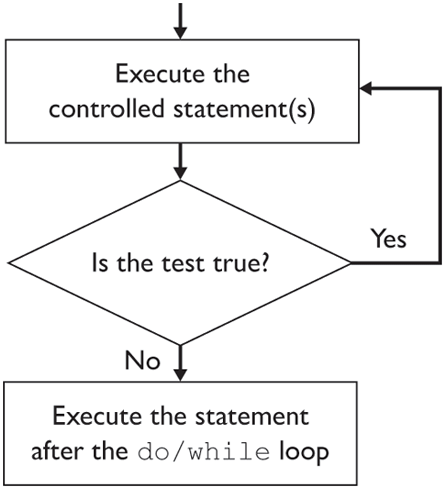
\includegraphics[max width=\linewidth]{Pictures/ch05_p25_img0.png}
\end{center}

Vòng lặp \texttt{do/while} hữu ích nhất trong các tình huống mà bạn biết mình phải thực thi vòng lặp ít nhất một lần. Ví dụ, trong phần trước chúng ta đã viết đoạn mã sau để mô phỏng việc tung hai con xúc xắc cho đến khi bạn có tổng bằng 7:

\begin{verbatim}
Random r = new Random();
int sum = 0; // đặt thành 0 để đảm bảo chúng ta vào vòng lặp
while (sum != 7) {
    // tung xúc xắc một lần
    int roll1 = r.nextInt(6) + 1;
    int roll2 = r.nextInt(6) + 1;
    sum = roll1 + roll2;
    System.out.println(roll1 + " + " + roll2 + " = " + sum);
}
\end{verbatim}

Chúng ta đã phải chuẩn bị trước cho vòng lặp bằng cách đặt \texttt{sum} thành 0 để máy tính đi vào vòng lặp. Với vòng lặp \texttt{do/while}, chúng ta có thể loại bỏ bước chuẩn bị này:

\begin{verbatim}
Random r = new Random();
int sum;
do {
    // tung xúc xắc một lần
    int roll1 = r.nextInt(6) + 1;
    int roll2 = r.nextInt(6) + 1;
    sum = roll1 + roll2;
    System.out.println(roll1 + " + " + roll2 + " = " + sum);
} while (sum != 7);
\end{verbatim}

Trong phiên bản này, chúng ta luôn thực thi thân vòng lặp ít nhất một lần, điều này giúp gán một giá trị cho biến \texttt{sum} trước khi nó đi tới điều kiện kiểm tra vòng lặp hiện xuất hiện ở đáy vòng lặp.

Có nhiều bài toán lập trình mà việc sử dụng vòng lặp \texttt{do/while} là phù hợp. Các vòng lặp này thường hữu ích trong các chương trình tương tác khi bạn biết mình muốn thực hiện một việc gì đó ít nhất một lần. Ví dụ: bạn có thể có một vòng lặp cho phép người dùng chơi một trò chơi nhiều lần; bạn có thể khá chắc chắn rằng người dùng sẽ muốn chơi ít nhất một lần. Tương tự như thế, nếu bạn đang chơi một trò chơi đoán số với người dùng, bạn sẽ luôn phải nhận được ít nhất một lượt đoán.

\subsection*{5.2 Thuật toán hàng rào (Fencepost Algorithms)}

Một bài toán lập trình phổ biến liên quan đến một loại vòng lặp đặc biệt được gọi là vòng lặp hàng rào (fencepost loop). Hãy xem xét bài toán sau: Bạn muốn dựng một hàng rào dài 100 yard, và bạn muốn lắp một cây cột (post) sau mỗi 10 yard. Bạn cần bao nhiêu cây cột? Nếu bạn nhẩm nhanh một phép chia trong đầu, bạn có thể nghĩ rằng mình cần 10 cây cột, nhưng thực tế bạn cần 11 cây cột. Đó là vì hàng rào bắt đầu và kết thúc bằng các cây cột. Nói cách khác, một hàng rào trông giống như Hình 5.3.

Hình 5.3 Một hàng rào điển hình

Vì bạn muốn có cột ở cả ngoài cùng bên trái và ngoài cùng bên phải, bạn không thể sử dụng vòng lặp đơn giản sau đây (nó không dựng cây cột cuối cùng):

\begin{verbatim}
for (chiều dài hàng rào) {
    dựng một cây cột.
    gắn một đoạn dây kẽm.
}
\end{verbatim}

Nếu bạn sử dụng vòng lặp trên, bạn sẽ có một hàng rào trông giống như Hình 5.4.

Hình 5.4 Một hàng rào bị lỗi

Việc thay đổi thứ tự của hai thao tác cũng không giải quyết được vấn đề, bởi vì khi đó bạn sẽ bỏ sót cây cột đầu tiên. Vấn đề với vòng lặp này là nó tạo ra số cây cột bằng đúng số đoạn dây kẽm, nhưng chúng ta biết rằng chúng ta cần thêm một cây cột nữa. Đó là lý do tại sao bài toán này đôi khi còn được gọi là bài toán "vòng lặp rưỡi" (loop and a half) — chúng ta muốn thực thi một nửa vòng lặp này (dựng một cây cột) thêm một lần nữa.
\section{Phần dịch trang 30 đến 40}
Một giải pháp là dựng một trong các cây cột trước hoặc sau vòng lặp (loop). Giải pháp thông thường là thực hiện việc đó trước:

\begin{verbatim}
dựng một cây cột.
for (chiều dài của hàng rào) {
    buộc một sợi dây thép.
    dựng một cây cột.
}
\end{verbatim}


Lưu ý rằng thứ tự của hai thao tác trong thân vòng lặp bây giờ đã được đảo ngược vì cây cột đầu tiên được dựng trước khi đi vào vòng lặp.

Một ví dụ đơn giản, hãy xem xét bài toán in ra các số nguyên từ 1 đến 10, phân tách bằng dấu phẩy. Nói cách khác, chúng ta muốn có kết quả đầu ra sau:
 
\begin{verbatim}
1, 2, 3, 4, 5, 6, 7, 8, 9, 10 
\end{verbatim}


Nhiệm vụ này là một bài toán hàng rào (fencepost problem) kinh điển vì chúng ta muốn in ra 10 con số nhưng chỉ có 9 dấu phẩy. Theo thuật ngữ hàng rào của chúng ta, việc ghi một con số là phần ``cột'' (post) của nhiệm vụ và ghi một dấu phẩy là phần ``dây thép'' (wire). Vì vậy, triển khai mã giả (pseudocode) mà chúng ta đã xây dựng, chúng ta in số đầu tiên trước vòng lặp và đảo ngược thứ tự các thao tác bên trong vòng lặp bằng cách in một dấu phẩy trước một con số:

\begin{verbatim}
System.out.print(1);
for (int i = 2; i <= 10; i++) {
    System.out.print(", " + i);
}
System.out.println();
\end{verbatim}


\subsection*{Hàng rào với if}

Nhiều vòng lặp hàng rào mà bạn viết sẽ yêu cầu thực thi có điều kiện. Trên thực tế, bản thân bài toán hàng rào có thể được giải quyết bằng một câu lệnh \texttt{if}. Hãy nhớ rằng giải pháp kinh điển cho bài toán hàng rào là xử lý cây cột đầu tiên trước khi vòng lặp bắt đầu:

\begin{verbatim}
dựng một cây cột.
for (chiều dài của hàng rào) {
    buộc một sợi dây thép.
    dựng một cây cột.
}
\end{verbatim}


Giải pháp này giải quyết được vấn đề, nhưng nó có thể gây bối rối vì bên trong vòng lặp, các bước dường như có thứ tự ngược lại. Bạn có thể sử dụng một câu lệnh \texttt{if} và giữ nguyên thứ tự ban đầu của các bước:

\begin{verbatim}
for (chiều dài của hàng rào) {
    dựng một cây cột.
    if (đây không phải là cây cột cuối cùng) {
        buộc một sợi dây thép.
    }
}
\end{verbatim}


Biến thể này không được sử dụng thường xuyên như giải pháp kinh điển vì nó liên quan đến cả điều kiện kiểm tra vòng lặp và điều kiện kiểm tra bên trong vòng lặp. Thường thì các kiểm tra này gần như giống hệt nhau, vì vậy việc kiểm tra cùng một thứ hai lần mỗi khi vòng lặp thực thi là không hiệu quả. Nhưng sẽ có những tình huống mà bạn có thể sử dụng cách tiếp cận này. Ví dụ, trong cách tiếp cận kinh điển, các dòng mã tương ứng với việc dựng một cây cột bị lặp lại. Nếu bạn đang viết một chương trình mà bước này đòi hỏi nhiều mã, bạn có thể quyết định rằng việc đặt câu lệnh \texttt{if} bên trong vòng lặp là một cách tiếp cận tốt hơn, ngay cả khi nó dẫn đến một số kiểm tra bổ sung.

Ví dụ, hãy xem xét việc viết một phương thức gọi là \texttt{multiprint} để in một chuỗi với một số lần cụ thể. Giả sử bạn muốn kết quả đầu ra nằm trên một dòng riêng biệt, bên trong dấu ngoặc vuông và được phân tách bằng dấu phẩy. Dưới đây là hai lệnh gọi ví dụ:

\begin{verbatim}
multiprint("please", 4);
multiprint("beetlejuice", 3);
\end{verbatim}


Bạn kỳ vọng những lệnh gọi này sẽ tạo ra kết quả đầu ra sau:
 
\begin{verbatim}
[please, please, please, please] 
[beetlejuice, beetlejuice, beetlejuice] 
\end{verbatim}


Nỗ lực đầu tiên của bạn trong việc viết phương thức này có thể là một vòng lặp đơn giản in các dấu ngoặc vuông bên ngoài vòng lặp và in chuỗi cùng dấu phẩy bên trong vòng lặp:

\begin{verbatim}
public static void multiprint(String s, int times) {
    System.out.print("[");
    for (int i = 1; i <= times; i++) {
        System.out.print(s + ", ");
    }
    System.out.println("]");
}
\end{verbatim}


Rất tiếc, đoạn mã này tạo ra một dấu phẩy thừa sau giá trị cuối cùng:
 
\begin{verbatim}
[please, please, please, please, ] 
[beetlejuice, beetlejuice, beetlejuice, ] 
\end{verbatim}


Bởi vì dấu phẩy là ký tự phân tách, bạn muốn số chuỗi in ra nhiều hơn số dấu phẩy một đơn vị (ví dụ: hai dấu phẩy để phân tách ba lần xuất hiện của ``beetlejuice''). Bạn có thể sử dụng giải pháp kinh điển cho bài toán hàng rào để đạt được hiệu ứng này bằng cách in một chuỗi bên ngoài vòng lặp và đảo ngược thứ tự in bên trong vòng lặp:

\begin{verbatim}
public static void multiprint(String s, int times) {
    System.out.print("[" + s);
    for (int i = 2; i <= times; i++) {
        System.out.print(", " + s);
    }
    System.out.println("]");
}
\end{verbatim}


Lưu ý rằng vì bạn đang in một trong các chuỗi trước khi vòng lặp bắt đầu, bạn phải sửa đổi vòng lặp để nó không in nhiều chuỗi như trước nữa. Việc điều chỉnh biến vòng lặp \texttt{i} bắt đầu từ hai sẽ bù cho giá trị đầu tiên được in trước vòng lặp.

Rất tiếc, giải pháp này cũng hoạt động không chính xác. Hãy xem xét điều gì xảy ra khi bạn yêu cầu phương thức in một chuỗi không lần (0 lần), như trong:

\begin{verbatim}
multiprint("please don't", 0);
\end{verbatim}


Lệnh gọi này tạo ra kết quả đầu ra không chính xác sau:
 
\begin{verbatim}
[please don't] 
\end{verbatim}


Bạn muốn người dùng có thể yêu cầu xuất hiện không lần một chuỗi, vì vậy phương thức không nên tạo ra kết quả đầu ra không chính xác đó. Vấn đề là giải pháp kinh điển cho bài toán hàng rào liên quan đến việc in một giá trị trước khi vòng lặp bắt đầu. Để phương thức hoạt động chính xác cho trường hợp bằng không, bạn có thể bao gồm một câu lệnh \texttt{if/else}:

\begin{verbatim}
public static void multiprint(String s, int times) {
    if (times == 0) {
        System.out.println("[]");

    } else {
        System.out.print("[" + s);
        for (int i = 2; i <= times; i++) {
            System.out.print(", " + s);
        }
        System.out.println("]");
    }
}
\end{verbatim}


Ngoài ra, bạn có thể bao gồm một câu lệnh \texttt{if} bên trong vòng lặp (cách tiếp cận kiểm tra kép):

\begin{verbatim}
public static void multiprint(String s, int times) {
    System.out.print("[");
    for (int i = 1; i <= times; i++) {
        System.out.print(s);
        if (i < times) {
            System.out.print(", ");
        }
    }
    System.out.println("]");
}
\end{verbatim}


Mặc dù phiên bản mã trước đó thực hiện một phép kiểm tra tương tự hai lần trong mỗi lần lặp, nhưng nó đơn giản hơn so với việc sử dụng giải pháp hàng rào kinh điển và trường hợp đặc biệt của nó. Không có giải pháp nào tốt hơn giải pháp nào, vì luôn có sự đánh đổi. Nếu bạn nghĩ rằng mã sẽ được thực thi thường xuyên và vòng lặp sẽ lặp lại nhiều lần, bạn có thể có xu hướng sử dụng giải pháp hiệu quả hơn. Ngược lại, bạn có thể chọn mã đơn giản hơn.

\subsection*{Vòng lặp Sentinel (Sentinel Loops)}

Giả sử bạn muốn đọc một loạt số từ người dùng và tính tổng của chúng. Bạn có thể hỏi trước người dùng xem cần đọc bao nhiêu số, như chúng ta đã làm trong chương trước, nhưng điều đó không phải lúc nào cũng thuận tiện. Điều gì sẽ xảy ra nếu người dùng có một danh sách dài các số cần nhập và chưa đếm chúng? Một cách để tránh việc hỏi số lượng là chọn một giá trị nhập đặc biệt để báo hiệu kết thúc nhập liệu. Chúng tôi gọi đây là giá trị lính canh (sentinel value).

\paragraph{Sentinel (Lính canh)}
Một giá trị đặc biệt báo hiệu kết thúc nhập liệu.

Ví dụ, bạn có thể yêu cầu người dùng nhập giá trị $-1$ để dừng nhập số. Nhưng làm thế nào để bạn cấu trúc mã của mình để sử dụng lính canh này? Nói chung, bạn sẽ muốn sử dụng cách tiếp cận sau:

\begin{verbatim}
sum = 0.
while (chúng ta chưa thấy lính canh) {
    nhắc và đọc giá trị.
    cộng nó vào tổng.
}
\end{verbatim}


Cách tiếp cận này không hoàn toàn hoạt động tốt. Ví dụ, giả sử người dùng nhập các số $10$, $42$, $5$ và $-1$. Như mã giả chỉ ra, chúng ta sẽ nhắc và đọc từng giá trị trong số bốn giá trị này rồi cộng chúng vào tổng cho đến khi gặp giá trị lính canh $-1$. Chúng ta khởi tạo tổng bằng $0$, vì vậy phép tính này tính $(10 + 42 + 5 + (-1))$, bằng $56$. Nhưng câu trả lời đúng phải là $57$. Giá trị lính canh $-1$ không được phép tính vào tổng.

Bài toán này là một bài toán hàng rào (fencepost) hoặc ``vòng lặp rưỡi'' (loop-and-a-half) kinh điển: Bạn muốn nhắc và đọc một loạt số, bao gồm cả lính canh, và bạn muốn cộng hầu hết các số lại, nhưng bạn không muốn cộng lính canh vào tổng.

Giải pháp hàng rào thông thường hoạt động hiệu quả: Chúng ta chèn câu lệnh nhắc-và-đọc đầu tiên trước vòng lặp và đảo ngược thứ tự của hai bước trong thân vòng lặp:

\begin{verbatim}
sum = 0.
nhắc và đọc giá trị.
while (chúng ta chưa thấy lính canh) {
    cộng nó vào tổng.
    nhắc và đọc giá trị.
}
\end{verbatim}


Sau đó, bạn có thể tinh chỉnh mã giả này bằng cách đưa vào một biến cho số được đọc từ người dùng:

\begin{verbatim}
sum = 0.
nhắc và đọc một giá trị vào n.
while (n không phải là lính canh) {
    cộng n vào tổng.
\end{verbatim}


\section{Phần dịch trang 40 đến 50}
yêu cầu nhập và đọc một giá trị vào n.


Đoạn mã giả (pseudocode) này được chuyển đổi khá dễ dàng sang mã Java như sau:

\begin{verbatim}
Scanner console = new Scanner(System.in);
int sum = 0;
System.out.print("next integer (–1 to quit)? ");
int number = console.nextInt();
while (number != –1) {
    sum += number;
    System.out.print("next integer (–1 to quit)? ");
    number = console.nextInt();
}
System.out.println("sum = " + sum);
\end{verbatim}


Khi đoạn mã trên được thực thi, quá trình tương tác có thể trông như thế này:

\begin{verbatim}
next integer (–1 to quit)? 10 
next integer (–1 to quit)? 20 
next integer (–1 to quit)? 30 
next integer (–1 to quit)? 40 
next integer (–1 to quit)? 50 
\end{verbatim}

next integer (–1 to quit)? 60 
next integer (–1 to quit)? –1 
sum = 210 


Một số học sinh nhận thấy rằng chương trình sẽ hoạt động tương tự nếu thay vì có một câu lệnh nhắc và đọc trước khi vòng lặp (loop) bắt đầu, chúng ta lại khởi tạo biến \texttt{number} bằng 0. Điều đó đúng trong trường hợp đặc biệt này, nhưng nó không mang tính tổng quát. Ví dụ, nếu bạn muốn tính giá trị lớn nhất (maximum) hoặc nhỏ nhất (minimum), bạn sẽ không muốn đưa số 0 vào làm một giá trị để xem xét. Vì vậy, mặc dù đoạn mã cụ thể này có thể được đơn giản hóa, chúng tôi vẫn muốn trình bày một giải pháp hoạt động hiệu quả cho tất cả các tác vụ tích lũy (cumulative tasks).

\subsection*{5.3 Kiểu boolean (The boolean Type)}

George Boole là một nhà logic học xuất sắc đến nỗi Java đã đặt tên một kiểu dữ liệu theo tên ông. Kiểu dữ liệu \texttt{boolean} trong Java được sử dụng để mô tả các mối quan hệ logic đúng/sai (true/false). Hãy nhớ lại rằng \texttt{boolean} là một trong các kiểu dữ liệu nguyên thủy (primitive types), giống như \texttt{int}, \texttt{double}, và \texttt{char}.

Những người mới bắt đầu thường thắc mắc tại sao các nhà khoa học máy tính lại quan tâm đến logic nhiều đến vậy. Câu trả lời là logic là nền tảng của ngành máy tính giống như vật lý là nền tảng của ngành kỹ thuật. Các kỹ sư học vật lý vì họ muốn chế tạo các vật thể trong thế giới thực vốn bị chi phối bởi các định luật vật lý. Nếu bạn không hiểu vật lý, bạn có khả năng sẽ xây dựng một cây cầu bị sập. Các nhà khoa học máy tính cũng xây dựng các sản phẩm, nhưng trong một thế giới ảo bị chi phối bởi các định luật logic. Nếu bạn không hiểu logic, bạn có khả năng sẽ viết ra các chương trình máy tính bị đổ vỡ.

Mà không hề nhận ra, bạn đã sử dụng các giá trị boolean rồi. Tất cả các cấu trúc điều khiển mà chúng ta đã xem xét—câu lệnh \texttt{if/else}, vòng lặp \texttt{for} (for loops), và vòng lặp \texttt{while} (while loops)—đều được điều khiển bởi các biểu thức xác định các điều kiện kiểm tra. Ví dụ, biểu thức
\begin{verbatim}
number % 2 == 0
\end{verbatim}

là một phép kiểm tra tính chia hết cho 2. Nó cũng là một biểu thức Boolean. Các biểu thức Boolean được thiết kế để nắm bắt các khái niệm về tính đúng và sai, vì vậy không có gì ngạc nhiên khi miền giá trị của kiểu \texttt{boolean} chỉ có hai giá trị: \texttt{true} (đúng) và \texttt{false} (sai). Các từ \texttt{true} và \texttt{false} là các từ khóa dành riêng (reserved words) trong Java. Chúng là các giá trị hằng (literals) của kiểu \texttt{boolean}. Tất cả các biểu thức Boolean, khi được đánh giá, sẽ trả về một trong hai giá trị hằng này. Đừng nhầm lẫn các giá trị đặc biệt này với các hằng chuỗi (string literals) \texttt{"true"} và \texttt{"false"}. Bạn không cần dấu ngoặc kép để tham chiếu đến các hằng Boolean.

Khi bạn viết một chương trình xử lý các giá trị số, bạn thường muốn tính toán một giá trị và lưu trữ nó vào một biến hoặc viết một phương thức (method) để thể hiện một công thức phức tạp nào đó. Chúng ta cũng làm điều tương tự với kiểu \texttt{boolean}. Chúng ta có thể muốn ghi lại một giá trị Boolean vào một biến và chúng ta thường viết các phương thức trả về kết quả Boolean. Ví dụ, chúng ta đã thấy lớp \texttt{String} có các phương thức trả về kết quả Boolean, bao gồm \texttt{startsWith}, \texttt{endsWith}, \texttt{equals}, và \texttt{equalsIgnoreCase}.

Để hiểu rõ hơn về điều này, hãy nhớ lại ý nghĩa của các thuật ngữ này đối với kiểu \texttt{int}. Các hằng (literals) của kiểu \texttt{int} bao gồm \texttt{0}, \texttt{1}, \texttt{2}, v.v. Bởi vì đây là các hằng của kiểu \texttt{int}, bạn có thể viết các biểu thức như sau với chúng:
\begin{verbatim}
int number1 = 1;
int number2 = 0;
\end{verbatim}


Hãy xem xét những gì bạn có thể làm với các biến kiểu \texttt{boolean}. Giả sử bạn định nghĩa hai biến \texttt{boolean}, \texttt{test1} và \texttt{test2}. Các biến này chỉ có thể nhận hai giá trị khả dĩ: \texttt{true} và \texttt{false}. Bạn có thể viết:
\begin{verbatim}
boolean test1 = true;
boolean test2 = false;
\end{verbatim}


Bạn cũng có thể viết một câu lệnh sao chép giá trị của một biến \texttt{boolean} này sang một biến khác, giống như với các biến thuộc bất kỳ kiểu dữ liệu nào khác:
\begin{verbatim}
test1 = test2;
\end{verbatim}


Hơn nữa, bạn biết rằng câu lệnh gán có thể sử dụng các biểu thức như:
\begin{verbatim}
number1 = 2 + 2;
\end{verbatim}

và rằng các phép kiểm tra đơn giản mà bạn đã và đang sử dụng là các biểu thức Boolean. Điều đó có nghĩa là bạn có thể viết các câu lệnh như sau:
\begin{verbatim}
test1 = (2 + 2 == 4);
test2 = (3 * 100 < 250);
\end{verbatim}


Các câu lệnh gán này, về mặt hiệu quả, có nghĩa là "Hãy đặt biến boolean này theo giá trị chân trị được trả về bởi phép kiểm tra sau." Câu lệnh đầu tiên đặt biến \texttt{test1} thành \texttt{true}, vì phép kiểm tra được đánh giá là đúng (\texttt{true}). Câu lệnh thứ hai đặt biến \texttt{test2} thành \texttt{false}, vì phép kiểm tra thứ hai được đánh giá là sai (\texttt{false}). Bạn không cần phải đưa vào các dấu ngoặc đơn, nhưng chúng làm cho các câu lệnh dễ đọc hơn. Rõ ràng, phép gán là một trong những thao tác bạn có thể thực hiện trên các biến kiểu \texttt{boolean}.

\subsection*{Toán tử logic (Logical Operators)}

Trong Java, bạn có thể tạo ra các biểu thức Boolean phức tạp bằng cách sử dụng các toán tử logic (logical operators), được hiển thị trong Bảng 5.3.

\noindent \textbf{Bảng 5.3: Các toán tử logic}

Toán tử phủ định NOT (\texttt{!}) đảo ngược giá trị chân trị của toán hạng của nó. Nếu một biểu thức có giá trị là \texttt{true}, phép phủ định của nó sẽ có giá trị là \texttt{false}, và ngược lại. Bạn có thể biểu diễn mối quan hệ này trong một bảng chân trị (truth table). Bảng chân trị sau đây có hai cột, một cột dành cho biến và một cột dành cho phủ định của nó. Đối với mỗi giá trị của biến, bảng hiển thị giá trị tương ứng của phép phủ định.

\noindent \textbf{Bảng chân trị cho phép phủ định NOT (\texttt{!})}

Ngoài toán tử phủ định, có hai phép liên kết logic mà bạn sẽ sử dụng là AND (\texttt{\&\&}) và OR (\texttt{||}). Bạn sử dụng các liên kết này để ràng buộc hai biểu thức Boolean lại với nhau, tạo ra một biểu thức Boolean mới. Bảng chân trị sau đây cho thấy toán tử AND chỉ được đánh giá là \texttt{true} khi cả hai toán hạng riêng lẻ của nó đều là \texttt{true}.

\noindent \textbf{Bảng chân trị cho phép AND (\texttt{\&\&})}

Bảng chân trị sau đây cho thấy toán tử OR được đánh giá là \texttt{true} ngoại trừ khi cả hai toán hạng đều là \texttt{false}.

\noindent \textbf{Bảng chân trị cho phép OR (\texttt{||})}

Toán tử OR trong Java có ý nghĩa hơi khác một chút so với từ "or" (hoặc) trong tiếng Anh thông thường. Trong tiếng Anh, bạn nói: "Tối nay tôi sẽ học bài hoặc tôi sẽ đi xem phim." Một trong hai điều sẽ đúng, nhưng không phải cả hai. Toán tử OR giống với cụm từ "và/hoặc" (and/or) hơn: Nếu một hoặc cả hai toán hạng là \texttt{true}, thì toàn bộ mệnh đề là \texttt{true}.

Bạn thường sử dụng các toán tử logic khi những gì bạn cần biểu diễn không thể rút gọn thành một phép kiểm tra đơn lẻ. Ví dụ, như chúng ta đã thấy ở chương trước, nếu bạn muốn thực hiện một thao tác cụ thể khi một số nằm trong khoảng từ 1 đến 10, bạn có thể viết:
\begin{verbatim}
if (number >= 1) {
    if (number <= 10) {
        doSomething();
    }
\end{verbatim}


Nhưng bạn có thể diễn đạt điều này dễ dàng hơn bằng cách sử dụng toán tử logic AND:
\begin{verbatim}
if (number >= 1 && number <= 10) {
    doSomething();
\end{verbatim}


Mọi người sử dụng các từ "và" và "hoặc" mọi lúc, nhưng Java chỉ cho phép bạn sử dụng chúng theo nghĩa logic chặt chẽ. Hãy cẩn thận để không viết mã như sau:
\begin{verbatim}
// đoạn mã này không biên dịch được
if (x == 1 || 2 || 3) {
    doSomething();
\end{verbatim}


Trong tiếng Anh thông thường, chúng ta sẽ đọc câu này là "x bằng 1 hoặc 2 hoặc 3", điều này có lý với chúng ta, nhưng lại không có nghĩa đối với Java. Bạn cũng có thể bị cám dỗ viết đoạn mã như sau:
\begin{verbatim}
// đoạn mã này không biên dịch được
if (1 <= x <= 10) {
    doSomethingElse();
\end{verbatim}


Trong toán học, biểu thức này sẽ có nghĩa và sẽ kiểm tra xem \texttt{x} có nằm trong khoảng từ 1 đến 10 (bao gồm cả hai đầu mút) hay không. Tuy nhiên, biểu thức này không có nghĩa trong Java.

Bạn chỉ có thể sử dụng các toán tử logic AND và OR để kết hợp một chuỗi các biểu thức Boolean. Nếu không, máy tính sẽ không hiểu ý bạn muốn diễn đạt. Để biểu diễn ý tưởng "1 hoặc 2 hoặc 3", hãy kết hợp ba biểu thức Boolean khác nhau bằng các toán tử logic OR:
\begin{verbatim}
if (x == 1 || x == 2 || x == 3) {
    doSomething();
\end{verbatim}


Để biểu diễn ý tưởng "nằm trong khoảng từ 1 đến 10 bao gồm cả hai đầu mút", hãy kết hợp hai biểu thức Boolean bằng một toán tử logic AND:
\begin{verbatim}
if (1 <= x && x <= 10) {
    doSomethingElse();
\end{verbatim}


Bây giờ chúng ta đã tìm hiểu về các toán tử logic AND, OR, và NOT, đã đến lúc xem xét lại bảng thứ tự ưu tiên (precedence table) của chúng ta. Toán tử NOT xuất hiện ở trên cùng, với mức độ ưu tiên cao nhất. Hai toán tử logic còn lại có mức độ ưu tiên khá thấp, thấp hơn các toán tử số học và quan hệ nhưng cao hơn các toán tử gán. Toán tử AND có mức độ ưu tiên cao hơn một chút so với toán tử OR. Bảng 5.4 bao gồm các toán tử mới này.

\noindent \textbf{Bảng 5.4: Thứ tự ưu tiên của toán tử trong Java}
\section{Phần dịch trang 50 đến 60}
Theo các quy tắc thứ tự ưu tiên này, khi Java đánh giá một biểu thức như biểu thức dưới đây, máy tính sẽ đánh giá toán tử NOT trước, tiếp theo là AND, và sau đó là OR.

\begin{verbatim}
if (test1 || !test2 && test3) {
    doSomething();
}
\end{verbatim}

\subsection*{Đánh giá ngắn mạch (Short-Circuited Evaluation)}

Trong phần này, chúng ta sẽ khám phá việc sử dụng các toán tử logic để giải quyết một tác vụ lập trình phức tạp, và chúng ta sẽ giới thiệu một thuộc tính quan trọng của các toán tử này. Chúng ta sẽ viết một phương thức tên là \texttt{firstWord} nhận vào một \texttt{String} làm tham số và trả về từ đầu tiên trong chuỗi đó. Để mọi thứ đơn giản, chúng ta quy ước rằng một \texttt{String} được phân tách thành các từ riêng lẻ bằng các khoảng trắng. Nếu \texttt{String} hoàn toàn không có từ nào, phương thức sẽ trả về một chuỗi rỗng. Dưới đây là một số ví dụ gọi hàm:

Hãy nhớ rằng chúng ta có thể gọi phương thức \texttt{substring} để trích xuất một phần của chuỗi. Chúng ta truyền hai tham số vào phương thức \texttt{substring}: chỉ số bắt đầu (starting index) của chuỗi con và chỉ số lớn hơn chỉ số kết thúc một đơn vị. Nếu chuỗi được lưu trữ trong một biến tên là \texttt{s}, nhiệm vụ của chúng ta cơ bản được rút gọn thành các bước sau:
\begin{itemize}
    \item đặt \texttt{start} thành chỉ số đầu tiên của từ.
    \item đặt \texttt{stop} thành chỉ số ngay sau từ đó.
    \item trả về \texttt{s.substring(start, stop)}.
\end{itemize}

Để tiếp cận bước đầu, hãy giả định rằng chỉ số bắt đầu là 0. Chỉ số bắt đầu này sẽ không hoạt động đối với các chuỗi bắt đầu bằng các khoảng trắng, nhưng nó sẽ cho phép chúng ta tập trung vào bước thứ hai trong mã giả (pseudocode).

Hãy xem xét một chuỗi bắt đầu bằng \texttt{"four score"}. Nếu chúng ta kiểm tra các ký tự riêng lẻ của chuỗi và chỉ số của chúng, chúng ta sẽ thấy mẫu sau:

Chúng ta đặt \texttt{start} thành 0. Chúng ta muốn đặt biến \texttt{stop} thành chỉ số ngay sau từ đầu tiên kết thúc. Trong ví dụ này, từ chúng ta muốn lấy là \texttt{"four"}, và nó kéo dài từ chỉ số 0 đến 3. Vì vậy, nếu chúng ta muốn biến \texttt{stop} lớn hơn chỉ số kết thúc một đơn vị, chúng ta muốn đặt nó thành chỉ số 4, vị trí của khoảng trắng đầu tiên trong chuỗi.

Vậy làm thế nào để chúng ta tìm thấy khoảng trắng đầu tiên trong chuỗi? Chúng ta sử dụng một vòng lặp (loop) \texttt{while}. Chúng ta chỉ cần bắt đầu từ đầu chuỗi và lặp cho đến khi gặp một khoảng trắng:
\begin{itemize}
    \item đặt \texttt{stop} thành 0.
    \item trong khi (ký tự tại chỉ số \texttt{stop} không phải là khoảng trắng) \{
    \begin{itemize}
        \item tăng \texttt{stop} lên 1.
    \end{itemize}
    \}
\end{itemize}

Điều này có thể dễ dàng chuyển đổi thành mã Java. Kết hợp nó với giả định của chúng ta rằng \texttt{start} sẽ bằng 0, chúng ta có:

\begin{verbatim}
public static String firstWord(String s) {
    int start = 0;
    int stop = 0;
    while (s.charAt(stop) != ' ') {
        stop++;
    }
    return s.substring(start, stop);
}
\end{verbatim}

Phiên bản này của phương thức hoạt động trong nhiều trường hợp, bao gồm cả chuỗi mẫu của chúng ta, nhưng nó không hoạt động với mọi chuỗi. Nó có hai hạn chế lớn. Chúng ta đã bắt đầu bằng cách giả định rằng chuỗi không bắt đầu bằng khoảng trắng, vì vậy chúng ta biết mình phải khắc phục hạn chế đó.

Vấn đề thứ hai là phiên bản \texttt{firstWord} này không hoạt động trên các chuỗi chỉ có một từ. Ví dụ, nếu chúng ta thực thi nó với một chuỗi như \texttt{"four"}, nó sẽ tạo ra một ngoại lệ \texttt{StringIndex\allowbreak{}OutOfBounds\allowbreak{}Exception} chỉ ra rằng 4 không phải là một chỉ số hợp lệ. Ngoại lệ xảy ra vì mã của chúng ta giả định rằng cuối cùng chúng ta sẽ tìm thấy một khoảng trắng, nhưng không có khoảng trắng nào trong chuỗi \texttt{"four"}. Vì vậy, \texttt{stop} được tăng lên cho đến khi bằng 4, và một ngoại lệ được ném ra vì không có ký tự nào ở chỉ số 4. Điều này đôi khi được gọi là ``vượt quá giới hạn cuối của chuỗi'' (running off the end of the string).

Để giải quyết vấn đề này, chúng ta cần kết hợp một điều kiện kiểm tra liên quan đến độ dài của chuỗi. Nhiều người mới học lập trình cố gắng thực hiện điều này bằng cách sử dụng một số sự kết hợp của \texttt{while} và \texttt{if}, như trong đoạn mã sau:

\begin{verbatim}
int stop = 0;
while (stop < s.length()) {
    if (s.charAt(stop) != ' ') {
       stop++;
    }
}
\end{verbatim}

Đoạn mã này hoạt động đối với các chuỗi một từ như \texttt{"four"} vì ngay khi \texttt{stop} bằng độ dài của chuỗi, chúng ta sẽ thoát ra khỏi vòng lặp. Tuy nhiên, nó không hoạt động đối với các trường hợp nhiều từ ban đầu như \texttt{"four score"}. Chúng ta kết thúc trong một vòng lặp vô hạn (infinite loop) vì một khi \texttt{stop} bằng 4, chúng ta ngừng tăng nó, nhưng chúng ta lại bị mắc kẹt bên trong vòng lặp vì điều kiện kiểm tra yêu cầu tiếp tục miễn là \texttt{stop} nhỏ hơn độ dài của chuỗi. Cách tiếp cận đặt một câu lệnh \texttt{if} bên trong một vòng lặp \texttt{while} này đã dẫn đến một lỗi nổi tiếng thế giới vào ngày 31 tháng 12 năm 2008, khi các máy nghe nhạc Zune trên toàn thế giới ngừng hoạt động (xem Bài tập tự kiểm tra 21 để biết thêm chi tiết).

Điểm cần nhận ra là trong trường hợp này chúng ta cần sử dụng hai điều kiện khác nhau để kiểm soát vòng lặp. Chúng ta chỉ muốn tiếp tục tăng \texttt{stop} nếu chúng ta biết rằng mình chưa gặp khoảng trắng và chưa đi đến cuối chuỗi. Chúng ta có thể thể hiện ý tưởng đó bằng cách sử dụng toán tử logic AND (\texttt{\&\&}):

\begin{verbatim}
int stop = 0;
while (s.charAt(stop) != ' ' && stop < s.length()) {
    stop++;
}
\end{verbatim}

Thật không may, ngay cả điều kiện kiểm tra này cũng không hoạt động. Nó thể hiện đúng hai điều kiện, vì chúng ta muốn đảm bảo rằng mình chưa gặp khoảng trắng và chúng ta muốn đảm bảo rằng mình chưa đi đến cuối chuỗi. Nhưng hãy nghĩ xem điều gì xảy ra ngay khi chúng ta chạm đến cuối chuỗi. Giả sử \texttt{s} là \texttt{"four"} và \texttt{stop} bằng 3.

Chúng ta thấy ký tự tại chỉ số 3 không phải là khoảng trắng và chúng ta thấy \texttt{stop} nhỏ hơn độ dài của chuỗi, vì vậy chúng ta tăng thêm một lần nữa và \texttt{stop} trở thành 4. Khi chúng ta quay lại vòng lặp, chúng ta kiểm tra xem \texttt{s.charAt(4)} có phải là khoảng trắng hay không. Việc kiểm tra này ném ra một ngoại lệ vì chỉ số nằm ngoài giới hạn. Chúng ta cũng kiểm tra xem \texttt{stop} có nhỏ hơn 4 hay không, điều này không đúng, nhưng việc kiểm tra đó diễn ra quá muộn để tránh ngoại lệ.

Java cung cấp một giải pháp cho tình huống này. Các toán tử logic \texttt{\&\&} và \texttt{||} sử dụng cơ chế đánh giá ngắn mạch (short-circuited evaluation).

\paragraph{Đánh giá ngắn mạch (Short-Circuited Evaluation)}
Thuộc tính của các toán tử logic \texttt{\&\&} và \texttt{||} giúp ngăn toán hạng thứ hai bị đánh giá nếu kết quả tổng thể đã rõ ràng từ giá trị của toán hạng đầu tiên.

Trong trường hợp của chúng ta, chúng ta đang thực hiện hai kiểm tra khác nhau và yêu cầu phép AND logic của hai kiểm tra đó. Nếu một trong hai kiểm tra thất bại, kết quả tổng thể sẽ là \texttt{false}, vì vậy nếu kiểm tra đầu tiên thất bại, không cần thiết phải thực hiện kiểm tra thứ hai. Do đánh giá ngắn mạch—nghĩa là vì kết quả tổng thể đã rõ ràng từ kiểm tra đầu tiên—chúng ta hoàn toàn không thực hiện kiểm tra thứ hai. Nói cách khác, việc thực hiện và đánh giá kiểm tra thứ hai bị ngăn chặn (ngắn mạch) bởi thực tế là kiểm tra đầu tiên đã thất bại.

Điều này có nghĩa là chúng ta cần đảo ngược thứ tự của hai kiểm tra này:

\begin{verbatim}
int stop = 0;
while (stop < s.length() && s.charAt(stop) != ' ') {
    stop++;
}
\end{verbatim}

Nếu chúng ta chạy lại kịch bản tương tự với \texttt{stop} bằng 3, chúng ta vượt qua cả hai bài kiểm tra này và tăng \texttt{stop} lên 4. Sau đó, khi quay lại vòng lặp một lần nữa, trước tiên chúng ta kiểm tra xem \texttt{stop} có nhỏ hơn \texttt{s.length()} hay không. Điều này không đúng, nghĩa là phép kiểm tra trả về giá trị \texttt{false}. Kết quả là, Java biết rằng biểu thức tổng thể sẽ có kết quả là \texttt{false} và không bao giờ đánh giá phép kiểm tra thứ hai. Thứ tự sự kiện này ngăn chặn ngoại lệ xảy ra, vì chúng ta không bao giờ kiểm tra xem \texttt{s.charAt(4)} có phải là khoảng trắng hay không.

Giải pháp này cung cấp cho chúng ta phiên bản thứ hai của phương thức:

\begin{verbatim}
public static String firstWord(String s) {
    int start = 0;
    int stop = 0;
    while (stop < s.length() && s.charAt(stop) != ' ') {
        stop++;
    }
    return s.substring(start, stop);
}
\end{verbatim}

Nhưng hãy nhớ rằng chúng ta đã giả định từ đầu tiên bắt đầu ở vị trí 0. Điều đó không nhất thiết luôn đúng. Ví dụ, nếu chúng ta truyền một chuỗi bắt đầu bằng nhiều khoảng trắng, phương thức này sẽ trả về một chuỗi rỗng. Chúng ta cần sửa đổi mã nguồn để nó bỏ qua bất kỳ khoảng trắng dẫn đầu nào. Để đạt được mục tiêu đó yêu cầu một vòng lặp khác. Để tiếp cận bước đầu, chúng ta có thể viết đoạn mã sau:

\begin{verbatim}
int start = 0;
while (s.charAt(start) == ' ') {
    start++;
}
\end{verbatim}

Đoạn mã này hoạt động đối với hầu hết các chuỗi, nhưng nó thất bại trong hai trường hợp quan trọng. Phép kiểm tra vòng lặp giả định rằng chúng ta sẽ tìm thấy một ký tự không phải khoảng trắng. Điều gì xảy ra nếu chuỗi hoàn toàn chứa các khoảng trắng? Trong trường hợp đó, chúng ta sẽ chỉ đơn giản là chạy quá giới hạn cuối của chuỗi, tạo ra một ngoại lệ \texttt{StringIndex\allowbreak{}OutOfBounds\allowbreak{}Exception}. Và điều gì xảy ra nếu ngay từ đầu chuỗi đã trống? Chúng ta sẽ gặp lỗi ngay lập tức khi chúng ta truy vấn \texttt{s.charAt(0)}, bởi vì không có ký tự nào ở chỉ số 0.

Chúng ta có thể quyết định rằng những trường hợp này cấu thành lỗi. Sau cùng, làm thế nào bạn có thể trả về từ đầu tiên nếu không có từ nào? Vì vậy, chúng ta có thể tài liệu hóa một tiền điều kiện (precondition) rằng chuỗi phải chứa ít nhất một ký tự không phải khoảng trắng, và ném ra một ngoại lệ nếu chúng ta thấy rằng nó không thỏa mãn. Một cách tiếp cận khác là trả về một chuỗi rỗng trong các trường hợp này.

Để giải quyết khả năng chuỗi có thể trống, chúng ta cần sửa đổi vòng lặp của mình để kết hợp phép kiểm tra độ dài của chuỗi. Nếu chúng ta thêm nó vào cuối kiểm tra vòng lặp \texttt{while} của mình, chúng ta có đoạn mã sau:

\begin{verbatim}
int start = 0;
while (s.charAt(start) == ' ' && start < s.length()) {
    start++;
}
\end{verbatim}

Nhưng đoạn mã này có cùng một khuyết điểm như chúng ta đã thấy trước đây. Nó được cho là để ngăn ngừa các vấn đề khi \texttt{start} bằng độ dài của chuỗi, nhưng khi tình huống này xảy ra, một \texttt{StringIndex\allowbreak{}OutOfBounds\allowbreak{}Exception} sẽ được ném ra trước khi máy tính thực hiện kiểm tra độ dài của chuỗi. Vì vậy, các phép kiểm tra này cũng phải được đảo ngược để tận dụng cơ chế đánh giá ngắn mạch:

\begin{verbatim}
int start = 0;
while (start < s.length() && s.charAt(start) == ' ') {
    start++;
}
\end{verbatim}

Để kết hợp các dòng mã này với mã trước đó của chúng ta, chúng ta phải thay đổi việc khởi tạo \texttt{stop}. Chúng ta không còn muốn tìm kiếm từ đầu chuỗi nữa. Thay vào đó, chúng ta cần khởi tạo \texttt{stop} bằng \texttt{start}. Ghép các phần này lại với nhau, chúng ta có được phiên bản phương thức sau:

\begin{verbatim}
public static String firstWord(String s) {
    int start = 0;
    while (start < s.length() && s.charAt(start) == ' ') {
        start++;
    }
    int stop = start;
    while (stop < s.length() && s.charAt(stop) != ' ') {
        stop++;
    }
    return s.substring(start, stop);
}
\end{verbatim}
\section{Phần dịch trang 60 đến 70}
Phiên bản này hoạt động trong mọi trường hợp, bỏ qua mọi khoảng trống dẫn đầu và trả về một chuỗi rỗng nếu không có từ nào để trả về.

\subsection*{Biến và Cờ boolean (boolean Variables and Flags)}

Tất cả các câu lệnh if/else đều được kiểm soát bởi các phép thử Boolean. Các phép thử này có thể là các biến boolean hoặc các biểu thức Boolean. Hãy xem xét ví dụ về đoạn mã sau:

\begin{verbatim}
if (number > 0) {
    System.out.println("positive");
} else {
    System.out.println("not positive");
}
\end{verbatim}

Đoạn mã này có thể được viết lại như sau:

\begin{verbatim}
boolean positive = (number > 0);
if (positive) {
    System.out.println("positive");
} else {

    System.out.println("not positive");
}
\end{verbatim}

Việc sử dụng các biến boolean giúp tăng khả năng đọc hiểu (readability) cho chương trình của bạn vì nó cho phép bạn đặt tên cho các phép thử. Hãy xem xét loại mã nguồn bạn sẽ tạo ra cho một chương trình hẹn hò. Bạn có thể có một số biến số nguyên mô tả các thuộc tính nhất định của một người: \texttt{looks}, để lưu trữ ước tính thô về vẻ đẹp ngoại hình (trên thang điểm từ 1--10); \texttt{IQ}, để lưu trữ chỉ số thông minh; \texttt{income}, để lưu trữ tổng thu nhập hàng năm; và \texttt{snothers}, để theo dõi những người bạn thân thiết ("snother" là viết tắt của "significant other" -- người đặc biệt). Với các biến này để xác định thuộc tính của một người, bạn có thể phát triển các phép thử mức độ phù hợp khác nhau. Khi viết chương trình, bạn có thể sử dụng các biến boolean để đặt tên cho các phép thử đó, giúp tăng đáng kể khả năng đọc hiểu của mã nguồn:

\begin{verbatim}
boolean cute = (looks >= 9);
boolean smart = (IQ > 125);
boolean rich = (income > 100000);
boolean available = (snothers == 0);
boolean awesome = cute && smart && rich && available;
\end{verbatim}

Đôi khi bạn sẽ có dịp sử dụng một loại biến boolean đặc biệt gọi là cờ (flag). Thông thường, chúng ta sử dụng các cờ bên trong các vòng lặp (loops) để ghi lại các điều kiện lỗi hoặc để báo hiệu sự hoàn thành. Các cờ khác nhau sẽ kiểm tra các điều kiện khác nhau. Như một phép ẩn dụ, hãy tưởng tượng một trọng tài trong một trận đấu thể thao, người theo dõi một hành vi phạm luật cụ thể và ném một chiếc cờ nếu điều đó xảy ra. Thỉnh thoảng bạn sẽ nghe thấy phát thanh viên nói rằng, "Đã có cờ báo lỗi trên sân."

Hãy đưa một chiếc cờ vào đoạn mã tính tổng tích lũy mà chúng ta đã thấy ở chương trước:

\begin{verbatim}
double sum = 0.0;
for (int i = 1; i <= totalNumber; i++) {
    System.out.print("    #" + i + "? ");
    double next = console.nextDouble();
    sum += next;
}
System.out.println("sum = " + sum);
\end{verbatim}

Giả sử chúng ta muốn biết liệu tổng số có bao giờ bị âm tại bất kỳ thời điểm nào hay không. Lưu ý rằng tình huống này không giống với tình huống tổng số cuối cùng nhận giá trị âm. Giống như số dư tài khoản ngân hàng, tổng số có thể chuyển đổi qua lại giữa dương và âm. Khi bạn thực hiện một chuỗi các giao dịch gửi và rút tiền, ngân hàng sẽ theo dõi xem bạn có từng rút quá số dư tài khoản của mình trong suốt quá trình đó hay không. Bằng cách sử dụng một cờ boolean, chúng ta có thể sửa đổi vòng lặp trước đó để theo dõi xem tổng số có bao giờ bị âm hay không và báo cáo kết quả sau vòng lặp:

\begin{verbatim}
double sum = 0.0;
boolean negative = false;
for (int i = 1; i <= totalNumber; i++) {
    System.out.print("    #" + i + "? ");
    double next = console.nextDouble();
    sum += next;
    if (sum < 0.0) {
        negative = true;
    }
}
System.out.println("sum = " + sum);
if (negative) {
    System.out.println("Sum went negative");
} else {
    System.out.println("Sum never went negative");
}
\end{verbatim}

Lưu ý rằng câu lệnh if bên trong vòng lặp không có nhánh else vì bạn không muốn đặt cờ trở lại giá trị \texttt{false} sau khi đã phát hiện một giá trị âm.

\subsection*{Thiền Boolean (Boolean Zen)}

Vào năm 1974, Robert Pirsig đã khởi xướng một xu hướng văn hóa với cuốn sách \textit{Zen and the Art of Motorcycle Maintenance: An Inquiry into Values} (Thiền và Nghệ thuật Bảo trì Xe máy: Một cuộc Truy vấn về các Giá trị). Một loạt sách sau đó đã sao chép tiêu đề này với cấu trúc \textit{Zen and the Art of X} (Thiền và Nghệ thuật của X), trong đó X là Poker, Đan lát, Viết lách, Bi lắc, Đàn Guitar, Giảng dạy ở Trường công, Kiếm sống, Yêu đương, May vá, Hài độc thoại, Kỳ thi SAT, Cắm hoa, Buộc mồi câu, Phân tích Hệ thống, Làm cha, Viết kịch bản, Kiểm soát Bệnh tiểu đường, Sự thân mật, Giúp đỡ, Đánh nhau trên đường phố, Giết người, và vân vân. Thậm chí còn có một cuốn sách mang tên \textit{Zen and the Art of Anything} (Thiền và Nghệ thuật của Mọi thứ).

Bây giờ chúng ta sẽ tham gia vào xu hướng văn hóa này bằng cách thảo luận về Thiền và nghệ thuật của kiểu dữ liệu \texttt{boolean}. Dường như nhiều người mới bắt đầu phải mất một thời gian để làm quen với các biểu thức Boolean. Những người mới bắt đầu thường viết các biểu thức quá phức tạp liên quan đến các giá trị boolean vì họ chưa nắm được sự đơn giản có thể đạt được khi bạn thực sự "hiểu" cách kiểu \texttt{boolean} hoạt động.

Ví dụ, giả sử bạn đang viết một chương trình trò chơi liên quan đến các số có hai chữ số, trong đó mỗi số được cấu tạo từ hai chữ số khác nhau. Nói cách khác, chương trình sẽ sử dụng các số như 42 được cấu tạo từ hai chữ số riêng biệt, chứ không sử dụng các số như 6 (chỉ có một chữ số), 394 (nhiều hơn hai chữ số), hoặc 22 (cả hai chữ số giống nhau). Bạn có thể muốn kiểm tra xem một số cho trước có hợp lệ để sử dụng trong trò chơi hay không. Bạn có thể giới hạn phạm vi trong các số có hai chữ số bằng một phép thử như sau:

\begin{verbatim}
n >= 10 && n <= 99
\end{verbatim}

Bạn cũng phải kiểm tra để đảm bảo rằng hai chữ số đó không giống nhau. Bạn có thể lấy các chữ số của một số có hai chữ số bằng các biểu thức \texttt{n / 10} và \texttt{n \% 10}. Vì vậy, bạn có thể mở rộng phép thử để đảm bảo rằng các chữ số không giống nhau:

\begin{verbatim}
n >= 10 && n <= 99 && (n / 10 != n % 10)
\end{verbatim}

Phép thử này là một ví dụ điển hình cho tình huống mà bạn có thể sử dụng một phương thức (method) để bao bọc một biểu thức Boolean phức tạp. Việc trả về một giá trị boolean sẽ cho phép bạn gọi phương thức đó bao nhiêu lần tùy thích mà không cần phải sao chép biểu thức phức tạp này mỗi lần, và bạn có thể đặt tên cho phép toán này để giúp chương trình dễ đọc hơn.

Giả sử bạn muốn gọi phương thức \texttt{isTwoUniqueDigits}. Bạn muốn phương thức này nhận một giá trị kiểu \texttt{int} và trả về \texttt{true} nếu số \texttt{int} đó được cấu tạo từ hai chữ số duy nhất và \texttt{false} nếu không phải. Do đó, phương thức sẽ trông như thế này:

\begin{verbatim}
public static boolean isTwoUniqueDigits(int n) {
    ...
}
\end{verbatim}

Bạn sẽ viết phần thân (body) của phương thức này như thế nào? Chúng ta đã viết xong phép thử, vì vậy chúng ta chỉ cần tìm cách tích hợp nó vào phương thức. Phương thức có kiểu trả về là boolean, nên bạn muốn nó trả về giá trị \texttt{true} khi phép thử thành công và giá trị \texttt{false} khi nó thất bại. Bạn có thể viết phương thức như sau:

\begin{verbatim}
public static boolean isTwoUniqueDigits(int n) {
    if (n >= 10 && n <= 99 && (n % 10 != n / 10)) {
        return true;
    } else {
        return false;
    }
}
\end{verbatim}

Phương thức này hoạt động tốt, nhưng nó dài dòng hơn mức cần thiết. Đoạn mã trên đánh giá phép thử mà chúng ta đã phát triển. Biểu thức đó có kiểu \texttt{boolean}, nghĩa là nó sẽ cho kết quả là \texttt{true} hoặc \texttt{false}. Câu lệnh if/else yêu cầu máy tính trả về \texttt{true} nếu biểu thức được đánh giá là \texttt{true} và trả về \texttt{false} nếu nó được đánh giá là \texttt{false}. Nhưng tại sao lại phải sử dụng cấu trúc này? Nếu phương thức sẽ trả về \texttt{true} khi biểu thức được đánh giá là \texttt{true} và trả về \texttt{false} khi nó được đánh giá là \texttt{false}, bạn có thể trả về trực tiếp giá trị của biểu thức đó luôn:

\begin{verbatim}
public static boolean isTwoUniqueDigits(int n) {
    return (n >= 10 && n <= 99 && (n % 10 != n / 10));
}
\end{verbatim}

Ngay cả phiên bản trước đó cũng có thể được đơn giản hóa, vì các dấu ngoặc đơn là không bắt buộc (mặc dù chúng giúp làm rõ chính xác những gì phương thức sẽ trả về). Đoạn mã này đánh giá phép thử mà chúng ta đã phát triển để xác định xem một số có được cấu tạo từ hai chữ số duy nhất hay không và trả về kết quả (\texttt{true} nếu đúng, \texttt{false} nếu sai).

Hãy xem xét một phép ẩn dụ tương tự với các biểu thức số nguyên. Đối với một người hiểu rõ về Boolean Zen, phiên bản if/else của phương thức này trông cũng kỳ quặc như đoạn mã sau:

\begin{verbatim}
if (x == 1) {
    return 1;
} else if (x == 2) {
    return 2;
} else if (x == 3) {
    return 3;
} else if (x == 4) {
    return 4;
} else if (x == 5) {

    return 5;
}
\end{verbatim}

Nếu bạn luôn muốn trả về giá trị của \texttt{x}, bạn chỉ cần viết:

\begin{verbatim}
return x;
\end{verbatim}

Sự nhầm lẫn tương tự cũng có thể xảy ra khi sinh viên sử dụng các biến boolean. Trong phần trước, chúng ta đã xem xét một biến thể của thuật toán tính tổng tích lũy có sử dụng một biến boolean tên là \texttt{negative} để theo dõi xem liệu tổng số có bao giờ bị âm hay không. Sau đó, chúng ta đã sử dụng một câu lệnh if/else để in ra một thông báo báo cáo kết quả:

\begin{verbatim}
if (negative) {
    System.out.println("Sum went negative");
} else {
    System.out.println("Sum never went negative");
}
\end{verbatim}

Một số người mới bắt đầu sẽ viết đoạn mã này như sau:

\begin{verbatim}
if (negative == true) {

    System.out.println("Sum went negative");
} else {
    System.out.println("Sum never went negative");
}
\end{verbatim}

Phép so sánh này là không cần thiết vì câu lệnh if/else mong muốn một biểu thức kiểu \texttt{boolean} xuất hiện bên trong dấu ngoặc đơn. Một biến boolean đã thuộc kiểu dữ liệu phù hợp rồi, vì vậy chúng ta không cần phải kiểm tra xem nó có bằng \texttt{true} hay không; nó hoặc là \texttt{true} hoặc là không phải (trong trường hợp đó nó là \texttt{false}). Đối với một người hiểu rõ về Boolean Zen, phép thử trên có vẻ dư thừa giống như việc nói rằng:

\begin{verbatim}
if ((negative == true) == true) {
    ...
}
\end{verbatim}

Những người mới bắt đầu cũng thường viết các phép thử như sau:

\begin{verbatim}
if (negative == false) {
    ...
}
\end{verbatim}
Điều này có phần hợp lý vì phép kiểm tra đang thực hiện một việc hữu ích, đó là nó đảo ngược ý nghĩa của biến boolean (trả về giá trị \texttt{true} nếu biến là \texttt{false} và trả về \texttt{false} nếu biến là \texttt{true}). Nhưng toán tử phủ định được thiết kế để thực hiện việc chuyển đổi các giá trị boolean này, vì vậy phép kiểm tra này tốt hơn nên được viết như sau:

\begin{verbatim}
if (!negative) {
    ...
}
\end{verbatim}

Bạn nên làm quen với việc đọc dấu chấm than là ``not'' (phủ định), do đó phép kiểm tra này sẽ được đọc là ``nếu không phải là negative'' (if not negative). Đối với những người hiểu về Boolean Zen, đó là một cách diễn đạt ngắn gọn hơn cho phép kiểm tra so với việc kiểm tra xem \texttt{negative} có bằng \texttt{false} hay không.

\subsection*{Phủ định biểu thức Boolean (Negating Boolean Expressions)}

Các lập trình viên thường thấy mình cần phải tạo phủ định của một biểu thức Boolean phức tạp. Ví dụ, thông thường cách dễ nhất để suy luận về một vòng lặp (loop) là dựa trên điều kiện thoát khiến chúng ta muốn dừng vòng lặp, nhưng vòng lặp \texttt{while} lại yêu cầu chúng ta biểu diễn mã nguồn theo điều kiện tiếp tục. Giả sử bạn muốn viết một vòng lặp liên tục nhắc người dùng nhập một số nguyên cho đến khi số nguyên đó là số có hai chữ số. Vì các số có hai chữ số nằm trong khoảng từ 10 đến 99, bạn có thể sử dụng các dòng mã sau để kiểm tra xem một số có chính xác hai chữ số hay không:

\begin{verbatim}
number >= 10 && number <= 99
\end{verbatim}

Để đưa điều này vào một vòng lặp \texttt{while}, chúng ta phải đảo ngược phép kiểm tra vì phép kiểm tra của vòng lặp \texttt{while} là một phép kiểm tra tiếp tục. Nói cách cách khác, chúng ta muốn tiếp tục ở trong vòng lặp khi điều này không đúng (khi người dùng vẫn chưa cung cấp cho chúng ta một số có hai chữ số). Một cách tiếp cận là sử dụng toán tử logic NOT để phủ định biểu thức này:

\begin{verbatim}
while (!(number >= 10 && number <= 99))
\end{verbatim}

Lưu ý rằng chúng ta cần đặt toàn bộ biểu thức Boolean trong dấu ngoặc đơn và sau đó đặt toán tử NOT ở phía trước nó. Mặc dù cách tiếp cận này hoạt động được, nhưng nó thường bị coi là phong cách lập trình không tốt. Tốt nhất là nên đơn giản hóa biểu thức này.

Một phương pháp tổng quát để đơn giản hóa các biểu thức như vậy đã được chính thức hóa bởi nhà logic học người Anh Augustus De Morgan. Chúng ta có thể áp dụng một trong hai quy tắc được gọi là định luật De Morgan (De Morgan's laws).

Bảng 5.5 hiển thị các định luật De Morgan. Lưu ý rằng khi bạn phủ định một biểu thức Boolean, mỗi toán hạng sẽ bị phủ định ($p$ trở thành $!p$ và $q$ trở thành $!q$) và toán tử logic sẽ đảo ngược. Toán tử OR logic trở thành AND logic và ngược lại khi bạn tính toán phủ định.

\subsubsection*{Bảng 5.5: Định luật De Morgan (De Morgan's Laws)}

Chúng ta có thể sử dụng định luật De Morgan thứ nhất cho chương trình số có hai chữ số của mình vì chúng ta đang cố gắng tìm phủ định của một biểu thức liên quan đến toán tử AND logic. Thay vì viết:

\begin{verbatim}
while (!(number >= 10 && number <= 99))
\end{verbatim}

chúng ta có thể viết:

\begin{verbatim}
while (number < 10 || number > 99)
\end{verbatim}

Mỗi phép kiểm tra riêng lẻ đã được phủ định và toán tử AND đã được thay thế bằng toán tử OR.

Hãy cùng xem xét ví dụ thứ hai liên quan đến định luật De Morgan còn lại. Giả sử bạn muốn hỏi người dùng một câu hỏi và bạn muốn bắt buộc người dùng phải trả lời ``yes'' hoặc ``no''. Nếu bạn có một biến kiểu \texttt{String} tên là \texttt{response}, bạn có thể sử dụng phép kiểm tra sau để mô tả điều bạn muốn nhận giá trị true:

\begin{verbatim}
response.equals("yes") || response.equals("no")
\end{verbatim}

Nếu chúng ta đang viết một vòng lặp để tiếp tục đọc phản hồi cho đến khi biểu thức này trả về giá trị true, thì chúng ta muốn viết vòng lặp sao cho nó sử dụng phủ định của phép kiểm tra này. Vì vậy, một lần nữa, chúng ta có thể sử dụng toán tử NOT cho toàn bộ biểu thức:

\begin{verbatim}
while (!(response.equals("yes") || response.equals("no")))
\end{verbatim}

Một lần nữa, tốt nhất là nên đơn giản hóa biểu thức bằng cách sử dụng định luật De Morgan:

\begin{verbatim}
while (!response.equals("yes") && !response.equals("no"))
\end{verbatim}

\subsection*{5.4 Lỗi của người dùng (User Errors)}

Trong chương trước, bạn đã tìm hiểu rằng một thói quen lập trình tốt là suy nghĩ về các tiền điều kiện (preconditions) của một phương thức và đề cập đến chúng trong phần chú thích của phương thức đó. Bạn cũng đã biết rằng trong một số trường hợp, mã của bạn có thể ném ra các ngoại lệ (exceptions) nếu các tiền điều kiện bị vi phạm.

Khi viết các chương trình tương tác, cách tiếp cận đơn giản nhất là giả định rằng người dùng sẽ cung cấp đầu vào hợp lệ. Sau đó, bạn có thể ghi lại các tiền điều kiện của mình bằng tài liệu và ném ra các ngoại lệ khi đầu vào của người dùng không như mong đợi. Tuy nhiên, nhìn chung, tốt hơn là nên viết các chương trình không đưa ra các giả định về đầu vào của người dùng. Ví dụ, bạn đã thấy đối tượng \texttt{Scanner} có thể ném ra một ngoại lệ nếu người dùng nhập sai kiểu dữ liệu. Tốt hơn hết là viết các chương trình có thể xử lý các lỗi của người dùng. Các chương trình như vậy được gọi là có tính bền vững (robust).

\begin{quote}
\textbf{Robust (Bền vững):} Khả năng của một chương trình vẫn thực thi được ngay cả khi gặp dữ liệu không hợp lệ.
\end{quote}

Trong phần này, chúng ta sẽ tìm hiểu cách viết các chương trình tương tác có tính bền vững. Tuy nhiên, trước khi có thể viết mã nguồn bền vững, bạn phải hiểu một số chức năng đặc biệt của lớp \texttt{Scanner}.

\subsubsection*{Khả năng nhìn trước của Scanner (Scanner Lookahead)}

Lớp \texttt{Scanner} có các phương thức cho phép bạn thực hiện kiểm tra trước khi đọc một giá trị. Nói cách khác, nó cho phép bạn nhìn trước khi nhảy (look before you leap). Đối với mỗi phương thức ``next'' của lớp \texttt{Scanner}, có một phương thức ``has'' tương ứng cho bạn biết liệu bạn có thể thực hiện thao tác đó hay không.

Ví dụ, bạn sẽ thường muốn đọc một số nguyên \texttt{int} bằng đối tượng \texttt{Scanner}. Nhưng chuyện gì sẽ xảy ra nếu người dùng nhập một thứ khác không phải là số nguyên? \texttt{Scanner} có một phương thức tên là \texttt{hasNextInt} cho biết việc đọc một số nguyên có khả năng thực hiện được vào lúc này hay không. Để xác định xem có khả năng đó hay không, đối tượng \texttt{Scanner} sẽ nhìn vào token (mã báo) tiếp theo và kiểm tra xem liệu nó có thể được thông dịch thành một số nguyên hay không.

Chúng ta có xu hướng giải thích một số chuỗi ký tự nhất định thành các kiểu dữ liệu cụ thể, nhưng khi chúng ta đọc các token, chúng có thể được giải thích theo những cách khác nhau. Chương trình dưới đây sẽ cho phép chúng ta khám phá khái niệm này:

\begin{verbatim}
 1 // Prints the ways a token of input can be read by the Scanner.
 2 import java.util.*;
 3
 4 public class ExamineInput1 {
 5     public static void main(String[] args) {
 6         System.out.println("This program examines the ways");
 7         System.out.println("a token can be read.");
 8         System.out.println();
 9
10         Scanner console = new Scanner(System.in);
11
12         System.out.print("token? ");
13         System.out.println("  hasNextInt = " +
14                            console.hasNextInt());
15         System.out.println("  hasNextDouble = " +
16                            console.hasNextDouble());
17         System.out.println("  hasNext = " + console.hasNext());
18    }
19 }
\end{verbatim}

Hãy cùng xem một vài lượt chạy mẫu. Dưới đây là kết quả đầu ra của chương trình khi chúng ta nhập token \texttt{348}:

\begin{verbatim}
This program examines the ways 
a token can be read. 
 
token? 348 
  hasNextInt = true 
  hasNextDouble = true 
  hasNext = true 
\end{verbatim}

Đúng như bạn mong đợi, lệnh gọi \texttt{hasNextInt} trả về \texttt{true}, nghĩa là chúng ta có thể hiểu token này là một số nguyên. \texttt{Scanner} cũng cho phép chúng ta hiểu token này dưới dạng một số thực \texttt{double}, vì vậy \texttt{hasNextDouble} cũng trả về \texttt{true}. Nhưng hãy chú ý rằng \texttt{hasNext()} cũng trả về \texttt{true}. Kết quả đó có nghĩa là chúng ta có thể gọi phương thức \texttt{next} để đọc token này dưới dạng một chuỗi ký tự (\texttt{String}).

Đây là một lượt chạy khác, lần này dành cho token \texttt{348.2}:

\begin{verbatim}
This program examines the ways 
a token can be read. 
 
token? 348.2 
  hasNextInt = false 
  hasNextDouble = true 
  hasNext = true 
\end{verbatim}

Token này không thể hiểu là một số nguyên (\texttt{int}), nhưng nó có thể hiểu là một số thực (\texttt{double}) hoặc một chuỗi (\texttt{String}). Cuối cùng, hãy xem xét lượt chạy này đối với token \texttt{hello}:

\begin{verbatim}
This program examines the ways 
a token can be read. 
 
token? hello 
  hasNextInt = false 
  hasNextDouble = false 
  hasNext = true 
\end{verbatim}

Token \texttt{hello} không thể hiểu là một số nguyên (\texttt{int}) hoặc số thực (\texttt{double}); nó chỉ có thể hiểu là một chuỗi (\texttt{String}).

\subsubsection*{Xử lý lỗi của người dùng (Handling User Errors)}

Hãy xem xét đoạn mã sau:

\begin{verbatim}
Scanner console = new Scanner(System.in);
System.out.print("How old are you? ");
int age = console.nextInt();
\end{verbatim}

Điều gì xảy ra nếu người dùng nhập một thứ không phải là số nguyên? Nếu điều đó xảy ra, \texttt{Scanner} sẽ ném ra một ngoại lệ tại lệnh gọi phương thức \texttt{nextInt}. Ở phần trước, chúng ta đã thấy rằng mình có thể kiểm tra xem token tiếp theo có thể hiểu là một số nguyên hay không bằng cách sử dụng phương thức \texttt{hasNextInt}. Do đó, chúng ta có thể kiểm tra trước khi đọc một số nguyên xem liệu người dùng đã nhập giá trị phù hợp hay chưa.

Nếu người dùng nhập thứ gì đó không phải là số nguyên, chúng ta muốn hủy bỏ dữ liệu đầu vào đó, in ra một loại thông báo lỗi nào đó và yêu cầu nhập lại lần hai. Chúng ta muốn đoạn mã này thực thi trong một vòng lặp để tiếp tục hủy bỏ đầu vào và tạo thông báo lỗi khi cần thiết cho đến khi người dùng nhập dữ liệu hợp lệ.

Dưới đây là nỗ lực đầu tiên cho một giải pháp bằng mã giả (pseudocode):

\begin{verbatim}
while (người dùng chưa nhập một số nguyên) {
    yêu cầu nhập.
    hủy bỏ đầu vào.
    tạo một thông báo lỗi.
\end{verbatim}

